\documentclass[1p]{elsarticle_modified}
%\bibliographystyle{elsarticle-num}

%\usepackage[colorlinks]{hyperref}
%\usepackage{abbrmath_seonhwa} %\Abb, \Ascr, \Acal ,\Abf, \Afrak
\usepackage{amsfonts}
\usepackage{amssymb}
\usepackage{amsmath}
\usepackage{amsthm}
\usepackage{scalefnt}
\usepackage{amsbsy}
\usepackage{kotex}
\usepackage{caption}
\usepackage{subfig}
\usepackage{color}
\usepackage{graphicx}
\usepackage{xcolor} %% white, black, red, green, blue, cyan, magenta, yellow
\usepackage{float}
\usepackage{setspace}
\usepackage{hyperref}

\usepackage{tikz}
\usetikzlibrary{arrows}

\usepackage{multirow}
\usepackage{array} % fixed length table
\usepackage{hhline}

%%%%%%%%%%%%%%%%%%%%%
\makeatletter
\renewcommand*\env@matrix[1][\arraystretch]{%
	\edef\arraystretch{#1}%
	\hskip -\arraycolsep
	\let\@ifnextchar\new@ifnextchar
	\array{*\c@MaxMatrixCols c}}
\makeatother %https://tex.stackexchange.com/questions/14071/how-can-i-increase-the-line-spacing-in-a-matrix
%%%%%%%%%%%%%%%

\usepackage[normalem]{ulem}

\newcommand{\msout}[1]{\ifmmode\text{\sout{\ensuremath{#1}}}\else\sout{#1}\fi}
%SOURCE: \msout is \stkout macro in https://tex.stackexchange.com/questions/20609/strikeout-in-math-mode

\newcommand{\cancel}[1]{
	\ifmmode
	{\color{red}\msout{#1}}
	\else
	{\color{red}\sout{#1}}
	\fi
}

\newcommand{\add}[1]{
	{\color{blue}\uwave{#1}}
}

\newcommand{\replace}[2]{
	\ifmmode
	{\color{red}\msout{#1}}{\color{blue}\uwave{#2}}
	\else
	{\color{red}\sout{#1}}{\color{blue}\uwave{#2}}
	\fi
}

\newcommand{\Sol}{\mathcal{S}} %segment
\newcommand{\D}{D} %diagram
\newcommand{\A}{\mathcal{A}} %arc


%%%%%%%%%%%%%%%%%%%%%%%%%%%%%5 test

\def\sl{\operatorname{\textup{SL}}(2,\Cbb)}
\def\psl{\operatorname{\textup{PSL}}(2,\Cbb)}
\def\quan{\mkern 1mu \triangleright \mkern 1mu}

\theoremstyle{definition}
\newtheorem{thm}{Theorem}[section]
\newtheorem{prop}[thm]{Proposition}
\newtheorem{lem}[thm]{Lemma}
\newtheorem{ques}[thm]{Question}
\newtheorem{cor}[thm]{Corollary}
\newtheorem{defn}[thm]{Definition}
\newtheorem{exam}[thm]{Example}
\newtheorem{rmk}[thm]{Remark}
\newtheorem{alg}[thm]{Algorithm}

\newcommand{\I}{\sqrt{-1}}
\begin{document}

%\begin{frontmatter}
%
%\title{Boundary parabolic representations of knots up to 8 crossings}
%
%%% Group authors per affiliation:
%\author{Yunhi Cho} 
%\address{Department of Mathematics, University of Seoul, Seoul, Korea}
%\ead{yhcho@uos.ac.kr}
%
%
%\author{Seonhwa Kim} %\fnref{s_kim}}
%\address{Center for Geometry and Physics, Institute for Basic Science, Pohang, 37673, Korea}
%\ead{ryeona17@ibs.re.kr}
%
%\author{Hyuk Kim}
%\address{Department of Mathematical Sciences, Seoul National University, Seoul 08826, Korea}
%\ead{hyukkim@snu.ac.kr}
%
%\author{Seokbeom Yoon}
%\address{Department of Mathematical Sciences, Seoul National University, Seoul, 08826,  Korea}
%\ead{sbyoon15@snu.ac.kr}
%
%\begin{abstract}
%We find all boundary parabolic representation of knots up to 8 crossings.
%
%\end{abstract}
%\begin{keyword}
%    \MSC[2010] 57M25 
%\end{keyword}
%
%\end{frontmatter}

%\linenumbers
%\tableofcontents
%
\newcommand\colored[1]{\textcolor{white}{\rule[-0.35ex]{0.8em}{1.4ex}}\kern-0.8em\color{red} #1}%
%\newcommand\colored[1]{\textcolor{white}{ #1}\kern-2.17ex	\textcolor{white}{ #1}\kern-1.81ex	\textcolor{white}{ #1}\kern-2.15ex\color{red}#1	}

{\Large $\underline{12n_{0185}~(K12n_{0185})}$}

\setlength{\tabcolsep}{10pt}
\renewcommand{\arraystretch}{1.6}
\vspace{1cm}\begin{tabular}{m{100pt}>{\centering\arraybackslash}m{274pt}}
\multirow{5}{120pt}{
	\centering
	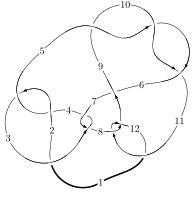
\includegraphics[width=112pt]{../../../GIT/diagram.site/Diagrams/png/2274_12n_0185.png}\\
\ \ \ A knot diagram\footnotemark}&
\allowdisplaybreaks
\textbf{Linearized knot diagam} \\
\cline{2-2}
 &
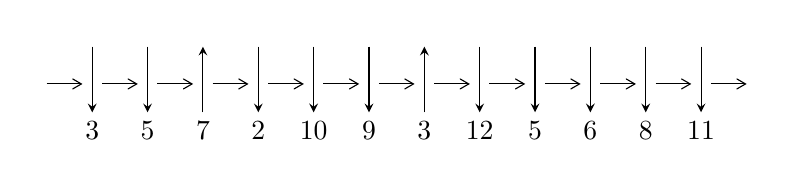
\begin{tikzpicture}[x=20pt, y=17pt]
	% nodes
	\node (C0) at (0, 0) {};
	\node (C1) at (1, 0) {};
	\node (C1U) at (1, +1) {};
	\node (C1D) at (1, -1) {3};

	\node (C2) at (2, 0) {};
	\node (C2U) at (2, +1) {};
	\node (C2D) at (2, -1) {5};

	\node (C3) at (3, 0) {};
	\node (C3U) at (3, +1) {};
	\node (C3D) at (3, -1) {7};

	\node (C4) at (4, 0) {};
	\node (C4U) at (4, +1) {};
	\node (C4D) at (4, -1) {2};

	\node (C5) at (5, 0) {};
	\node (C5U) at (5, +1) {};
	\node (C5D) at (5, -1) {10};

	\node (C6) at (6, 0) {};
	\node (C6U) at (6, +1) {};
	\node (C6D) at (6, -1) {9};

	\node (C7) at (7, 0) {};
	\node (C7U) at (7, +1) {};
	\node (C7D) at (7, -1) {3};

	\node (C8) at (8, 0) {};
	\node (C8U) at (8, +1) {};
	\node (C8D) at (8, -1) {12};

	\node (C9) at (9, 0) {};
	\node (C9U) at (9, +1) {};
	\node (C9D) at (9, -1) {5};

	\node (C10) at (10, 0) {};
	\node (C10U) at (10, +1) {};
	\node (C10D) at (10, -1) {6};

	\node (C11) at (11, 0) {};
	\node (C11U) at (11, +1) {};
	\node (C11D) at (11, -1) {8};

	\node (C12) at (12, 0) {};
	\node (C12U) at (12, +1) {};
	\node (C12D) at (12, -1) {11};
	\node (C13) at (13, 0) {};

	% arrows
	\draw[->,>={angle 60}]
	(C0) edge (C1) (C1) edge (C2) (C2) edge (C3) (C3) edge (C4) (C4) edge (C5) (C5) edge (C6) (C6) edge (C7) (C7) edge (C8) (C8) edge (C9) (C9) edge (C10) (C10) edge (C11) (C11) edge (C12) (C12) edge (C13) ;	\draw[->,>=stealth]
	(C1U) edge (C1D) (C2U) edge (C2D) (C3D) edge (C3U) (C4U) edge (C4D) (C5U) edge (C5D) (C6U) edge (C6D) (C7D) edge (C7U) (C8U) edge (C8D) (C9U) edge (C9D) (C10U) edge (C10D) (C11U) edge (C11D) (C12U) edge (C12D) ;
	\end{tikzpicture} \\
\hhline{~~} \\& 
\textbf{Solving Sequence} \\ \cline{2-2} 
 &
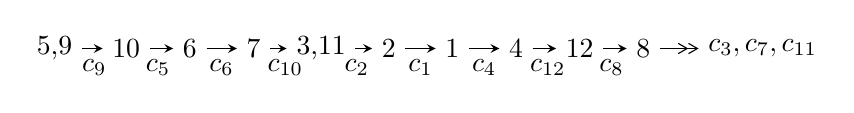
\begin{tikzpicture}[x=23pt, y=7pt]
	% node
	\node (A0) at (-1/8, 0) {5,9};
	\node (A1) at (1, 0) {10};
	\node (A2) at (2, 0) {6};
	\node (A3) at (3, 0) {7};
	\node (A4) at (65/16, 0) {3,11};
	\node (A5) at (41/8, 0) {2};
	\node (A6) at (49/8, 0) {1};
	\node (A7) at (57/8, 0) {4};
	\node (A8) at (65/8, 0) {12};
	\node (A9) at (73/8, 0) {8};
	\node (C1) at (1/2, -1) {$c_{9}$};
	\node (C2) at (3/2, -1) {$c_{5}$};
	\node (C3) at (5/2, -1) {$c_{6}$};
	\node (C4) at (7/2, -1) {$c_{10}$};
	\node (C5) at (37/8, -1) {$c_{2}$};
	\node (C6) at (45/8, -1) {$c_{1}$};
	\node (C7) at (53/8, -1) {$c_{4}$};
	\node (C8) at (61/8, -1) {$c_{12}$};
	\node (C9) at (69/8, -1) {$c_{8}$};
	\node (A10) at (11, 0) {$c_{3},c_{7},c_{11}$};

	% edge
	\draw[->,>=stealth]	
	(A0) edge (A1) (A1) edge (A2) (A2) edge (A3) (A3) edge (A4) (A4) edge (A5) (A5) edge (A6) (A6) edge (A7) (A7) edge (A8) (A8) edge (A9) ;
	\draw[->>,>={angle 60}]	
	(A9) edge (A10);
\end{tikzpicture} \\ 

\end{tabular} \\

\footnotetext{
The image of knot diagram is generated by the software ``\textbf{Draw programme}" developed by Andrew Bartholomew(\url{http://www.layer8.co.uk/maths/draw/index.htm\#Running-draw}), where we modified some parts for our purpose(\url{https://github.com/CATsTAILs/LinksPainter}).
}\phantom \\ \newline 
\centering \textbf{Ideals for irreducible components\footnotemark of $X_{\text{par}}$} 
 
\begin{align*}
I^u_{1}&=\langle 
376024023995393 u^{34}+337812687444816 u^{33}+\cdots+236220224312633 b-92299978153456,\\
\phantom{I^u_{1}}&\phantom{= \langle  }-21436667059562 u^{34}-138041311777599 u^{33}+\cdots+236220224312633 a-507133705138188,\\
\phantom{I^u_{1}}&\phantom{= \langle  }u^{35}+2 u^{34}+\cdots+7 u^2-1\rangle \\
I^u_{2}&=\langle 
- u^7- u^6+2 u^5+3 u^4-2 u^2+b-3 u-2,\;- u^7+u^6+3 u^5-2 u^4-3 u^3+a+2,\\
\phantom{I^u_{2}}&\phantom{= \langle  }u^8- u^7-3 u^6+2 u^5+3 u^4-2 u-1\rangle \\
\\
\end{align*}
\raggedright * 2 irreducible components of $\dim_{\mathbb{C}}=0$, with total 43 representations.\\
\footnotetext{All coefficients of polynomials are rational numbers. But the coefficients are sometimes approximated in decimal forms when there is not enough margin.}
\newpage
\renewcommand{\arraystretch}{1}
\centering \section*{I. $I^u_{1}= \langle 3.76\times10^{14} u^{34}+3.38\times10^{14} u^{33}+\cdots+2.36\times10^{14} b-9.23\times10^{13},\;-2.14\times10^{13} u^{34}-1.38\times10^{14} u^{33}+\cdots+2.36\times10^{14} a-5.07\times10^{14},\;u^{35}+2 u^{34}+\cdots+7 u^2-1 \rangle$}
\flushleft \textbf{(i) Arc colorings}\\
\begin{tabular}{m{7pt} m{180pt} m{7pt} m{180pt} }
\flushright $a_{5}=$&$\begin{pmatrix}0\\u\end{pmatrix}$ \\
\flushright $a_{9}=$&$\begin{pmatrix}1\\0\end{pmatrix}$ \\
\flushright $a_{10}=$&$\begin{pmatrix}1\\u^2\end{pmatrix}$ \\
\flushright $a_{6}=$&$\begin{pmatrix}- u\\- u^3+u\end{pmatrix}$ \\
\flushright $a_{7}=$&$\begin{pmatrix}u^3-2 u\\- u^3+u\end{pmatrix}$ \\
\flushright $a_{3}=$&$\begin{pmatrix}0.0907487 u^{34}+0.584376 u^{33}+\cdots+2.44395 u+2.14687\\-1.59184 u^{34}-1.43008 u^{33}+\cdots-0.811363 u+0.390737\end{pmatrix}$ \\
\flushright $a_{11}=$&$\begin{pmatrix}- u^2+1\\- u^4+2 u^2\end{pmatrix}$ \\
\flushright $a_{2}=$&$\begin{pmatrix}0.0907487 u^{34}+0.584376 u^{33}+\cdots+2.44395 u+2.14687\\-1.45102 u^{34}-1.18233 u^{33}+\cdots-0.902112 u-0.0121412\end{pmatrix}$ \\
\flushright $a_{1}=$&$\begin{pmatrix}0.575913 u^{34}+0.751783 u^{33}+\cdots+1.72764 u-0.721893\\0.273973 u^{34}+0.369123 u^{33}+\cdots+0.836448 u-1.01092\end{pmatrix}$ \\
\flushright $a_{4}=$&$\begin{pmatrix}-0.0507248 u^{34}+0.357239 u^{33}+\cdots+1.91500 u+2.35136\\-1.53287 u^{34}-1.32266 u^{33}+\cdots-0.588139 u+0.311133\end{pmatrix}$ \\
\flushright $a_{12}=$&$\begin{pmatrix}0.356599 u^{34}+0.653291 u^{33}+\cdots+1.26570 u-0.986457\\0.215125 u^{34}+0.426155 u^{33}+\cdots+0.736752 u-0.781963\end{pmatrix}$ \\
\flushright $a_{8}=$&$\begin{pmatrix}-0.722473 u^{34}-1.09863 u^{33}+\cdots-1.64586 u+1.70851\\0.119619 u^{34}+0.128063 u^{33}+\cdots-0.342320 u-0.375739\end{pmatrix}$\\&\end{tabular}
\flushleft \textbf{(ii) Obstruction class $= -1$}\\~\\
\flushleft \textbf{(iii) Cusp Shapes $= -\frac{2062473679663797}{236220224312633} u^{34}-\frac{828575186416011}{236220224312633} u^{33}+\cdots+\frac{1259833306856340}{236220224312633} u-\frac{231203744342586}{236220224312633}$}\\~\\
\newpage\renewcommand{\arraystretch}{1}
\flushleft \textbf{(iv) u-Polynomials at the component}\newline \\
\begin{tabular}{m{50pt}|m{274pt}}
Crossings & \hspace{64pt}u-Polynomials at each crossing \\
\hline $$\begin{aligned}c_{1}\end{aligned}$$&$\begin{aligned}
&u^{35}+49 u^{34}+\cdots+3150 u+1
\end{aligned}$\\
\hline $$\begin{aligned}c_{2},c_{4}\end{aligned}$$&$\begin{aligned}
&u^{35}-9 u^{34}+\cdots-70 u+1
\end{aligned}$\\
\hline $$\begin{aligned}c_{3},c_{7}\end{aligned}$$&$\begin{aligned}
&u^{35}-3 u^{34}+\cdots-2432 u-256
\end{aligned}$\\
\hline $$\begin{aligned}c_{5},c_{9},c_{10}\end{aligned}$$&$\begin{aligned}
&u^{35}+2 u^{34}+\cdots+7 u^2-1
\end{aligned}$\\
\hline $$\begin{aligned}c_{6}\end{aligned}$$&$\begin{aligned}
&u^{35}-6 u^{34}+\cdots+1364 u-847
\end{aligned}$\\
\hline $$\begin{aligned}c_{8},c_{11}\end{aligned}$$&$\begin{aligned}
&u^{35}+2 u^{34}+\cdots+4 u+1
\end{aligned}$\\
\hline $$\begin{aligned}c_{12}\end{aligned}$$&$\begin{aligned}
&u^{35}+24 u^{34}+\cdots+14 u+1
\end{aligned}$\\
\hline
\end{tabular}\\~\\
\newpage\renewcommand{\arraystretch}{1}
\flushleft \textbf{(v) Riley Polynomials at the component}\newline \\
\begin{tabular}{m{50pt}|m{274pt}}
Crossings & \hspace{64pt}Riley Polynomials at each crossing \\
\hline $$\begin{aligned}c_{1}\end{aligned}$$&$\begin{aligned}
&y^{35}-117 y^{34}+\cdots+9175798 y-1
\end{aligned}$\\
\hline $$\begin{aligned}c_{2},c_{4}\end{aligned}$$&$\begin{aligned}
&y^{35}-49 y^{34}+\cdots+3150 y-1
\end{aligned}$\\
\hline $$\begin{aligned}c_{3},c_{7}\end{aligned}$$&$\begin{aligned}
&y^{35}+51 y^{34}+\cdots+5423104 y-65536
\end{aligned}$\\
\hline $$\begin{aligned}c_{5},c_{9},c_{10}\end{aligned}$$&$\begin{aligned}
&y^{35}-36 y^{34}+\cdots+14 y-1
\end{aligned}$\\
\hline $$\begin{aligned}c_{6}\end{aligned}$$&$\begin{aligned}
&y^{35}-36 y^{34}+\cdots+23619926 y-717409
\end{aligned}$\\
\hline $$\begin{aligned}c_{8},c_{11}\end{aligned}$$&$\begin{aligned}
&y^{35}-24 y^{34}+\cdots+14 y-1
\end{aligned}$\\
\hline $$\begin{aligned}c_{12}\end{aligned}$$&$\begin{aligned}
&y^{35}-24 y^{34}+\cdots+402 y-1
\end{aligned}$\\
\hline
\end{tabular}\\~\\
\newpage\flushleft \textbf{(vi) Complex Volumes and Cusp Shapes}
$$\begin{array}{c|c|c}  
\text{Solutions to }I^u_{1}& \I (\text{vol} + \sqrt{-1}CS) & \text{Cusp shape}\\
 \hline 
\begin{aligned}
u &= -0.571697 + 0.825819 I \\
a &= \phantom{-}1.02997 + 1.33115 I \\
b &= -0.13854 - 1.61473 I\end{aligned}
 & -8.58737 + 2.74263 I & -10.41024 - 2.56572 I \\ \hline\begin{aligned}
u &= -0.571697 - 0.825819 I \\
a &= \phantom{-}1.02997 - 1.33115 I \\
b &= -0.13854 + 1.61473 I\end{aligned}
 & -8.58737 - 2.74263 I & -10.41024 + 2.56572 I \\ \hline\begin{aligned}
u &= \phantom{-}0.552087 + 0.825280 I \\
a &= -0.87268 + 1.55881 I \\
b &= -0.20679 - 1.66620 I\end{aligned}
 & -12.94840 + 3.24222 I & -12.66532 - 0.54583 I \\ \hline\begin{aligned}
u &= \phantom{-}0.552087 - 0.825280 I \\
a &= -0.87268 - 1.55881 I \\
b &= -0.20679 + 1.66620 I\end{aligned}
 & -12.94840 - 3.24222 I & -12.66532 + 0.54583 I \\ \hline\begin{aligned}
u &= \phantom{-}0.575473 + 0.807100 I \\
a &= -1.29277 + 1.27295 I \\
b &= \phantom{-}0.43025 - 1.79381 I\end{aligned}
 & -13.0318 - 8.6571 I & -12.52203 + 5.43059 I \\ \hline\begin{aligned}
u &= \phantom{-}0.575473 - 0.807100 I \\
a &= -1.29277 - 1.27295 I \\
b &= \phantom{-}0.43025 + 1.79381 I\end{aligned}
 & -13.0318 + 8.6571 I & -12.52203 - 5.43059 I \\ \hline\begin{aligned}
u &= -1.215130 + 0.192273 I \\
a &= \phantom{-}0.340293 + 0.190807 I \\
b &= -0.450734 + 0.019324 I\end{aligned}
 & -1.72471 + 0.87161 I & -4.58345 + 0.49262 I \\ \hline\begin{aligned}
u &= -1.215130 - 0.192273 I \\
a &= \phantom{-}0.340293 - 0.190807 I \\
b &= -0.450734 - 0.019324 I\end{aligned}
 & -1.72471 - 0.87161 I & -4.58345 - 0.49262 I \\ \hline\begin{aligned}
u &= -0.128163 + 0.673108 I \\
a &= -0.157665 + 0.722315 I \\
b &= \phantom{-}0.179473 - 0.037885 I\end{aligned}
 & \phantom{-}1.43459 + 2.27058 I & -1.42314 - 3.26969 I \\ \hline\begin{aligned}
u &= -0.128163 - 0.673108 I \\
a &= -0.157665 - 0.722315 I \\
b &= \phantom{-}0.179473 + 0.037885 I\end{aligned}
 & \phantom{-}1.43459 - 2.27058 I & -1.42314 + 3.26969 I\\
 \hline 
 \end{array}$$\newpage$$\begin{array}{c|c|c}  
\text{Solutions to }I^u_{1}& \I (\text{vol} + \sqrt{-1}CS) & \text{Cusp shape}\\
 \hline 
\begin{aligned}
u &= \phantom{-}0.521823 + 0.375425 I \\
a &= \phantom{-}1.98216 + 0.47145 I \\
b &= -0.419285 + 1.197250 I\end{aligned}
 & -4.17337 - 3.54764 I & -13.9483 + 7.1314 I \\ \hline\begin{aligned}
u &= \phantom{-}0.521823 - 0.375425 I \\
a &= \phantom{-}1.98216 - 0.47145 I \\
b &= -0.419285 - 1.197250 I\end{aligned}
 & -4.17337 + 3.54764 I & -13.9483 - 7.1314 I \\ \hline\begin{aligned}
u &= -0.628588\phantom{ +0.000000I} \\
a &= -2.61914\phantom{ +0.000000I} \\
b &= -0.676319\phantom{ +0.000000I}\end{aligned}
 & -6.22799\phantom{ +0.000000I} & -17.7300\phantom{ +0.000000I} \\ \hline\begin{aligned}
u &= \phantom{-}1.38882\phantom{ +0.000000I} \\
a &= -0.0130861\phantom{ +0.000000I} \\
b &= \phantom{-}1.19281\phantom{ +0.000000I}\end{aligned}
 & -6.53287\phantom{ +0.000000I} & -13.8260\phantom{ +0.000000I} \\ \hline\begin{aligned}
u &= \phantom{-}1.366140 + 0.266698 I \\
a &= -0.369885 + 0.416733 I \\
b &= \phantom{-}0.1060940 + 0.0070702 I\end{aligned}
 & -3.30368 - 5.68455 I & -8.00000 + 0. I\phantom{ +0.000000I} \\ \hline\begin{aligned}
u &= \phantom{-}1.366140 - 0.266698 I \\
a &= -0.369885 - 0.416733 I \\
b &= \phantom{-}0.1060940 - 0.0070702 I\end{aligned}
 & -3.30368 + 5.68455 I & -8.00000 + 0. I\phantom{ +0.000000I} \\ \hline\begin{aligned}
u &= -1.44080\phantom{ +0.000000I} \\
a &= -0.727727\phantom{ +0.000000I} \\
b &= \phantom{-}7.36351\phantom{ +0.000000I}\end{aligned}
 & -8.27744\phantom{ +0.000000I} & \phantom{-}27.9740\phantom{ +0.000000I} \\ \hline\begin{aligned}
u &= -1.47539\phantom{ +0.000000I} \\
a &= -0.857502\phantom{ +0.000000I} \\
b &= \phantom{-}2.36593\phantom{ +0.000000I}\end{aligned}
 & -8.21207\phantom{ +0.000000I} & -8.00000\phantom{ +0.000000I} \\ \hline\begin{aligned}
u &= \phantom{-}1.47608 + 0.08600 I \\
a &= \phantom{-}0.570629 + 0.485997 I \\
b &= -0.33599 + 1.45625 I\end{aligned}
 & -6.62003 - 2.59519 I & \phantom{-0.000000 } 0 \\ \hline\begin{aligned}
u &= \phantom{-}1.47608 - 0.08600 I \\
a &= \phantom{-}0.570629 - 0.485997 I \\
b &= -0.33599 - 1.45625 I\end{aligned}
 & -6.62003 + 2.59519 I & \phantom{-0.000000 } 0\\
 \hline 
 \end{array}$$\newpage$$\begin{array}{c|c|c}  
\text{Solutions to }I^u_{1}& \I (\text{vol} + \sqrt{-1}CS) & \text{Cusp shape}\\
 \hline 
\begin{aligned}
u &= -0.349636 + 0.351362 I \\
a &= -1.224010 - 0.204907 I \\
b &= \phantom{-}0.210574 + 0.830362 I\end{aligned}
 & -0.594132 + 1.120540 I & -6.95383 - 6.15774 I \\ \hline\begin{aligned}
u &= -0.349636 - 0.351362 I \\
a &= -1.224010 + 0.204907 I \\
b &= \phantom{-}0.210574 - 0.830362 I\end{aligned}
 & -0.594132 - 1.120540 I & -6.95383 + 6.15774 I \\ \hline\begin{aligned}
u &= -1.52553 + 0.10391 I \\
a &= -0.768523 + 0.940824 I \\
b &= \phantom{-}0.459596 + 1.316590 I\end{aligned}
 & -10.99510 + 5.24946 I & \phantom{-0.000000 } 0 \\ \hline\begin{aligned}
u &= -1.52553 - 0.10391 I \\
a &= -0.768523 - 0.940824 I \\
b &= \phantom{-}0.459596 - 1.316590 I\end{aligned}
 & -10.99510 - 5.24946 I & \phantom{-0.000000 } 0 \\ \hline\begin{aligned}
u &= \phantom{-}1.54711\phantom{ +0.000000I} \\
a &= \phantom{-}1.47176\phantom{ +0.000000I} \\
b &= -0.141707\phantom{ +0.000000I}\end{aligned}
 & -13.5056\phantom{ +0.000000I} & \phantom{-0.000000 } 0 \\ \hline\begin{aligned}
u &= \phantom{-}0.209346 + 0.398609 I \\
a &= \phantom{-}0.21466 - 2.09699 I \\
b &= \phantom{-}0.49858 + 1.79535 I\end{aligned}
 & -3.31433 + 0.90397 I & -10.45251 + 5.11287 I \\ \hline\begin{aligned}
u &= \phantom{-}0.209346 - 0.398609 I \\
a &= \phantom{-}0.21466 + 2.09699 I \\
b &= \phantom{-}0.49858 - 1.79535 I\end{aligned}
 & -3.31433 - 0.90397 I & -10.45251 - 5.11287 I \\ \hline\begin{aligned}
u &= -0.439838\phantom{ +0.000000I} \\
a &= \phantom{-}0.227233\phantom{ +0.000000I} \\
b &= -0.497327\phantom{ +0.000000I}\end{aligned}
 & -0.965385\phantom{ +0.000000I} & -10.6440\phantom{ +0.000000I} \\ \hline\begin{aligned}
u &= -1.56383 + 0.27842 I \\
a &= \phantom{-}1.192970 - 0.084215 I \\
b &= -0.57843 - 2.00327 I\end{aligned}
 & \phantom{-}19.4383 + 12.6641 I & \phantom{-0.000000 } 0 \\ \hline\begin{aligned}
u &= -1.56383 - 0.27842 I \\
a &= \phantom{-}1.192970 + 0.084215 I \\
b &= -0.57843 + 2.00327 I\end{aligned}
 & \phantom{-}19.4383 - 12.6641 I & \phantom{-0.000000 } 0\\
 \hline 
 \end{array}$$\newpage$$\begin{array}{c|c|c}  
\text{Solutions to }I^u_{1}& \I (\text{vol} + \sqrt{-1}CS) & \text{Cusp shape}\\
 \hline 
\begin{aligned}
u &= -1.56397 + 0.29270 I \\
a &= \phantom{-}1.145030 + 0.192290 I \\
b &= -0.07466 - 1.64853 I\end{aligned}
 & \phantom{-}19.6118 + 0.8962 I & \phantom{-0.000000 } 0 \\ \hline\begin{aligned}
u &= -1.56397 - 0.29270 I \\
a &= \phantom{-}1.145030 - 0.192290 I \\
b &= -0.07466 + 1.64853 I\end{aligned}
 & \phantom{-}19.6118 - 0.8962 I & \phantom{-0.000000 } 0 \\ \hline\begin{aligned}
u &= \phantom{-}1.56922 + 0.28522 I \\
a &= -1.121370 + 0.038644 I \\
b &= \phantom{-}0.40086 - 1.74127 I\end{aligned}
 & -15.6045 - 6.8496 I & \phantom{-0.000000 } 0 \\ \hline\begin{aligned}
u &= \phantom{-}1.56922 - 0.28522 I \\
a &= -1.121370 - 0.038644 I \\
b &= \phantom{-}0.40086 + 1.74127 I\end{aligned}
 & -15.6045 + 6.8496 I & \phantom{-0.000000 } 0 \\ \hline\begin{aligned}
u &= \phantom{-}0.344297\phantom{ +0.000000I} \\
a &= \phantom{-}3.18086\phantom{ +0.000000I} \\
b &= -0.768868\phantom{ +0.000000I}\end{aligned}
 & -2.11337\phantom{ +0.000000I} & \phantom{-}0.398900\phantom{ +0.000000I}\\
 \hline 
 \end{array}$$\newpage\newpage\renewcommand{\arraystretch}{1}
\centering \section*{II. $I^u_{2}= \langle - u^7- u^6+2 u^5+3 u^4-2 u^2+b-3 u-2,\;- u^7+u^6+3 u^5-2 u^4-3 u^3+a+2,\;u^8- u^7-3 u^6+2 u^5+3 u^4-2 u-1 \rangle$}
\flushleft \textbf{(i) Arc colorings}\\
\begin{tabular}{m{7pt} m{180pt} m{7pt} m{180pt} }
\flushright $a_{5}=$&$\begin{pmatrix}0\\u\end{pmatrix}$ \\
\flushright $a_{9}=$&$\begin{pmatrix}1\\0\end{pmatrix}$ \\
\flushright $a_{10}=$&$\begin{pmatrix}1\\u^2\end{pmatrix}$ \\
\flushright $a_{6}=$&$\begin{pmatrix}- u\\- u^3+u\end{pmatrix}$ \\
\flushright $a_{7}=$&$\begin{pmatrix}u^3-2 u\\- u^3+u\end{pmatrix}$ \\
\flushright $a_{3}=$&$\begin{pmatrix}u^7- u^6-3 u^5+2 u^4+3 u^3-2\\u^7+u^6-2 u^5-3 u^4+2 u^2+3 u+2\end{pmatrix}$ \\
\flushright $a_{11}=$&$\begin{pmatrix}- u^2+1\\- u^4+2 u^2\end{pmatrix}$ \\
\flushright $a_{2}=$&$\begin{pmatrix}u^7- u^6-3 u^5+2 u^4+3 u^3-2\\u^7+u^6-2 u^5-3 u^4+2 u^2+2 u+2\end{pmatrix}$ \\
\flushright $a_{1}=$&$\begin{pmatrix}0\\- u\end{pmatrix}$ \\
\flushright $a_{4}=$&$\begin{pmatrix}u^7- u^6-3 u^5+2 u^4+3 u^3-2\\u^7+u^6-2 u^5-3 u^4+2 u^2+3 u+2\end{pmatrix}$ \\
\flushright $a_{12}=$&$\begin{pmatrix}- u^5+2 u^3- u\\- u^7+3 u^5-2 u^3- u\end{pmatrix}$ \\
\flushright $a_{8}=$&$\begin{pmatrix}u^3-2 u\\- u^3+u\end{pmatrix}$\\&\end{tabular}
\flushleft \textbf{(ii) Obstruction class $= 1$}\\~\\
\flushleft \textbf{(iii) Cusp Shapes $= -4 u^7-9 u^6+10 u^5+27 u^4+2 u^3-18 u^2-20 u-29$}\\~\\
\newpage\renewcommand{\arraystretch}{1}
\flushleft \textbf{(iv) u-Polynomials at the component}\newline \\
\begin{tabular}{m{50pt}|m{274pt}}
Crossings & \hspace{64pt}u-Polynomials at each crossing \\
\hline $$\begin{aligned}c_{1},c_{2}\end{aligned}$$&$\begin{aligned}
&(u-1)^8
\end{aligned}$\\
\hline $$\begin{aligned}c_{3},c_{7}\end{aligned}$$&$\begin{aligned}
&u^8
\end{aligned}$\\
\hline $$\begin{aligned}c_{4}\end{aligned}$$&$\begin{aligned}
&(u+1)^8
\end{aligned}$\\
\hline $$\begin{aligned}c_{5}\end{aligned}$$&$\begin{aligned}
&u^8+u^7-3 u^6-2 u^5+3 u^4+2 u-1
\end{aligned}$\\
\hline $$\begin{aligned}c_{6}\end{aligned}$$&$\begin{aligned}
&u^8-3 u^7+7 u^6-10 u^5+11 u^4-10 u^3+6 u^2-4 u+1
\end{aligned}$\\
\hline $$\begin{aligned}c_{8}\end{aligned}$$&$\begin{aligned}
&u^8- u^7- u^6+2 u^5+u^4-2 u^3+2 u-1
\end{aligned}$\\
\hline $$\begin{aligned}c_{9},c_{10}\end{aligned}$$&$\begin{aligned}
&u^8- u^7-3 u^6+2 u^5+3 u^4-2 u-1
\end{aligned}$\\
\hline $$\begin{aligned}c_{11}\end{aligned}$$&$\begin{aligned}
&u^8+u^7- u^6-2 u^5+u^4+2 u^3-2 u-1
\end{aligned}$\\
\hline $$\begin{aligned}c_{12}\end{aligned}$$&$\begin{aligned}
&u^8+3 u^7+7 u^6+10 u^5+11 u^4+10 u^3+6 u^2+4 u+1
\end{aligned}$\\
\hline
\end{tabular}\\~\\
\newpage\renewcommand{\arraystretch}{1}
\flushleft \textbf{(v) Riley Polynomials at the component}\newline \\
\begin{tabular}{m{50pt}|m{274pt}}
Crossings & \hspace{64pt}Riley Polynomials at each crossing \\
\hline $$\begin{aligned}c_{1},c_{2},c_{4}\end{aligned}$$&$\begin{aligned}
&(y-1)^8
\end{aligned}$\\
\hline $$\begin{aligned}c_{3},c_{7}\end{aligned}$$&$\begin{aligned}
&y^8
\end{aligned}$\\
\hline $$\begin{aligned}c_{5},c_{9},c_{10}\end{aligned}$$&$\begin{aligned}
&y^8-7 y^7+19 y^6-22 y^5+3 y^4+14 y^3-6 y^2-4 y+1
\end{aligned}$\\
\hline $$\begin{aligned}c_{6},c_{12}\end{aligned}$$&$\begin{aligned}
&y^8+5 y^7+11 y^6+6 y^5-17 y^4-34 y^3-22 y^2-4 y+1
\end{aligned}$\\
\hline $$\begin{aligned}c_{8},c_{11}\end{aligned}$$&$\begin{aligned}
&y^8-3 y^7+7 y^6-10 y^5+11 y^4-10 y^3+6 y^2-4 y+1
\end{aligned}$\\
\hline
\end{tabular}\\~\\
\newpage\flushleft \textbf{(vi) Complex Volumes and Cusp Shapes}
$$\begin{array}{c|c|c}  
\text{Solutions to }I^u_{2}& \I (\text{vol} + \sqrt{-1}CS) & \text{Cusp shape}\\
 \hline 
\begin{aligned}
u &= -1.180120 + 0.268597 I \\
a &= -0.805639 - 0.183365 I \\
b &= \phantom{-}0.037144 + 0.630517 I\end{aligned}
 & -2.68559 + 1.13123 I & -13.38132 - 1.25921 I \\ \hline\begin{aligned}
u &= -1.180120 - 0.268597 I \\
a &= -0.805639 + 0.183365 I \\
b &= \phantom{-}0.037144 - 0.630517 I\end{aligned}
 & -2.68559 - 1.13123 I & -13.38132 + 1.25921 I \\ \hline\begin{aligned}
u &= -0.108090 + 0.747508 I \\
a &= -0.189481 - 1.310380 I \\
b &= \phantom{-}0.082879 + 0.802680 I\end{aligned}
 & \phantom{-}0.51448 + 2.57849 I & -10.25723 - 4.63100 I \\ \hline\begin{aligned}
u &= -0.108090 - 0.747508 I \\
a &= -0.189481 + 1.310380 I \\
b &= \phantom{-}0.082879 - 0.802680 I\end{aligned}
 & \phantom{-}0.51448 - 2.57849 I & -10.25723 + 4.63100 I \\ \hline\begin{aligned}
u &= \phantom{-}1.37100\phantom{ +0.000000I} \\
a &= \phantom{-}0.729394\phantom{ +0.000000I} \\
b &= \phantom{-}5.33104\phantom{ +0.000000I}\end{aligned}
 & -8.14766\phantom{ +0.000000I} & -37.4550\phantom{ +0.000000I} \\ \hline\begin{aligned}
u &= \phantom{-}1.334530 + 0.318930 I \\
a &= \phantom{-}0.708845 - 0.169402 I \\
b &= -0.259819 + 0.832925 I\end{aligned}
 & -4.02461 - 6.44354 I & -13.7170 + 7.8762 I \\ \hline\begin{aligned}
u &= \phantom{-}1.334530 - 0.318930 I \\
a &= \phantom{-}0.708845 + 0.169402 I \\
b &= -0.259819 - 0.832925 I\end{aligned}
 & -4.02461 + 6.44354 I & -13.7170 - 7.8762 I \\ \hline\begin{aligned}
u &= -0.463640\phantom{ +0.000000I} \\
a &= -2.15684\phantom{ +0.000000I} \\
b &= \phantom{-}0.948553\phantom{ +0.000000I}\end{aligned}
 & -2.48997\phantom{ +0.000000I} & -22.8330\phantom{ +0.000000I}\\
 \hline 
 \end{array}$$\newpage
\newpage\renewcommand{\arraystretch}{1}
\centering \section*{ III. u-Polynomials}
\begin{tabular}{m{50pt}|m{274pt}}
Crossings & \hspace{64pt}u-Polynomials at each crossing \\
\hline $$\begin{aligned}c_{1}\end{aligned}$$&$\begin{aligned}
&((u-1)^8)(u^{35}+49 u^{34}+\cdots+3150 u+1)
\end{aligned}$\\
\hline $$\begin{aligned}c_{2}\end{aligned}$$&$\begin{aligned}
&((u-1)^8)(u^{35}-9 u^{34}+\cdots-70 u+1)
\end{aligned}$\\
\hline $$\begin{aligned}c_{3},c_{7}\end{aligned}$$&$\begin{aligned}
&u^8(u^{35}-3 u^{34}+\cdots-2432 u-256)
\end{aligned}$\\
\hline $$\begin{aligned}c_{4}\end{aligned}$$&$\begin{aligned}
&((u+1)^8)(u^{35}-9 u^{34}+\cdots-70 u+1)
\end{aligned}$\\
\hline $$\begin{aligned}c_{5}\end{aligned}$$&$\begin{aligned}
&(u^8+u^7-3 u^6-2 u^5+3 u^4+2 u-1)(u^{35}+2 u^{34}+\cdots+7 u^2-1)
\end{aligned}$\\
\hline $$\begin{aligned}c_{6}\end{aligned}$$&$\begin{aligned}
&(u^8-3 u^7+7 u^6-10 u^5+11 u^4-10 u^3+6 u^2-4 u+1)\\
&\cdot(u^{35}-6 u^{34}+\cdots+1364 u-847)
\end{aligned}$\\
\hline $$\begin{aligned}c_{8}\end{aligned}$$&$\begin{aligned}
&(u^8- u^7+\cdots+2 u-1)(u^{35}+2 u^{34}+\cdots+4 u+1)
\end{aligned}$\\
\hline $$\begin{aligned}c_{9},c_{10}\end{aligned}$$&$\begin{aligned}
&(u^8- u^7-3 u^6+2 u^5+3 u^4-2 u-1)(u^{35}+2 u^{34}+\cdots+7 u^2-1)
\end{aligned}$\\
\hline $$\begin{aligned}c_{11}\end{aligned}$$&$\begin{aligned}
&(u^8+u^7+\cdots-2 u-1)(u^{35}+2 u^{34}+\cdots+4 u+1)
\end{aligned}$\\
\hline $$\begin{aligned}c_{12}\end{aligned}$$&$\begin{aligned}
&(u^8+3 u^7+7 u^6+10 u^5+11 u^4+10 u^3+6 u^2+4 u+1)\\
&\cdot(u^{35}+24 u^{34}+\cdots+14 u+1)
\end{aligned}$\\
\hline
\end{tabular}\newpage\renewcommand{\arraystretch}{1}
\centering \section*{ IV. Riley Polynomials}
\begin{tabular}{m{50pt}|m{274pt}}
Crossings & \hspace{64pt}Riley Polynomials at each crossing \\
\hline $$\begin{aligned}c_{1}\end{aligned}$$&$\begin{aligned}
&((y-1)^8)(y^{35}-117 y^{34}+\cdots+9175798 y-1)
\end{aligned}$\\
\hline $$\begin{aligned}c_{2},c_{4}\end{aligned}$$&$\begin{aligned}
&((y-1)^8)(y^{35}-49 y^{34}+\cdots+3150 y-1)
\end{aligned}$\\
\hline $$\begin{aligned}c_{3},c_{7}\end{aligned}$$&$\begin{aligned}
&y^8(y^{35}+51 y^{34}+\cdots+5423104 y-65536)
\end{aligned}$\\
\hline $$\begin{aligned}c_{5},c_{9},c_{10}\end{aligned}$$&$\begin{aligned}
&(y^8-7 y^7+19 y^6-22 y^5+3 y^4+14 y^3-6 y^2-4 y+1)\\
&\cdot(y^{35}-36 y^{34}+\cdots+14 y-1)
\end{aligned}$\\
\hline $$\begin{aligned}c_{6}\end{aligned}$$&$\begin{aligned}
&(y^8+5 y^7+11 y^6+6 y^5-17 y^4-34 y^3-22 y^2-4 y+1)\\
&\cdot(y^{35}-36 y^{34}+\cdots+23619926 y-717409)
\end{aligned}$\\
\hline $$\begin{aligned}c_{8},c_{11}\end{aligned}$$&$\begin{aligned}
&(y^8-3 y^7+7 y^6-10 y^5+11 y^4-10 y^3+6 y^2-4 y+1)\\
&\cdot(y^{35}-24 y^{34}+\cdots+14 y-1)
\end{aligned}$\\
\hline $$\begin{aligned}c_{12}\end{aligned}$$&$\begin{aligned}
&(y^8+5 y^7+11 y^6+6 y^5-17 y^4-34 y^3-22 y^2-4 y+1)\\
&\cdot(y^{35}-24 y^{34}+\cdots+402 y-1)
\end{aligned}$\\
\hline
\end{tabular}
\vskip 2pc
\end{document}